\documentclass[dvipdfmx,autodetect-engine,titlepage]{jsarticle}
\usepackage[dvipdfm]{graphicx}
\usepackage{ascmac}
\usepackage{fancybox}
\usepackage{listings}
\usepackage{plistings}
\usepackage{itembkbx}
\usepackage{amsmath}
\usepackage{url}
\usepackage{graphics}
\usepackage{listings}
\usepackage{here}

\lstset{%
  language={C},
  basicstyle={\small},%
  identifierstyle={\small},%
  commentstyle={\small\itshape\color[rgb]{0,0.5,0}},%
  keywordstyle={\small\bfseries\color[rgb]{0,0,1}},%
  ndkeywordstyle={\small},%
  stringstyle={\small\ttfamily\color[rgb]{1,0,1}},
  frame={tb},
  breaklines=true,
  columns=[l]{fullflexible},%
  numbers=left,%
  xrightmargin=0zw,%
  xleftmargin=3zw,%
  numberstyle={\scriptsize},%
  stepnumber=1,
  numbersep=1zw,%
  lineskip=-0.5ex%
}

\textheight=23cm
\renewcommand{\figurename}{図}
\renewcommand{\tablename}{表}
\newenvironment{code}
{\vspace{0.5zw}\VerbatimEnvironment  \begin{screen} 
\baselineskip=1.0\normalbaselineskip
 \begin{Verbatim}}
{\end{Verbatim}
\baselineskip=\normalbaselineskip
 \end{screen}\vspace{0.5zw}} 

\title{セキュリティ・ネットワーク学実験3\\
地上デジタル放送受信アンテナ制作\\
最終レポート
}
\author{2600200087-2\\Oku Wakana\\奥 若菜}
\date{May. 29 2022}

\begin{document}

\maketitle

\section{3-4th week 半波長ダイポールアンテナ}
\subsection{アンテナの概要}
半波長ダイポールアンテナは、2本の等しい長さのエレメントの間に給電点を持つ、全長1/2λのアンテナである。効率が良く、特性を簡単な計算でかなり正確に推定できることから、標準アンテナとして用いられる。
ここではABC朝日放送(482-488MHz帯)を受信することを目的としたアンテナを制作する。\\

\subsection{アンテナの設計}
ABC朝日放送の周波数範囲が482-488MHzであるので、中心周波数の485MHzで波長の計算を行った。

\begin{eqnarray*}
  \lambda = \frac{3.0 \times 10^8 [m/s]}{2.4 \times 10^8 [m/s]} = 0.618[m] = 61.8[cm]\\
\end{eqnarray*}

2本のエレメントの長さはそれぞれ1/4λなので、15.5cmでとなる。それに0.6cmの給電点を合わせた全体の長さが31.6cmのアンテナを設計した。
実際にモデリングしたものが下の図1である。また、このアンテナのモデリングは1セルを6mmと設定して行った。\\\\

\begin{figure}[H]
  \centering
  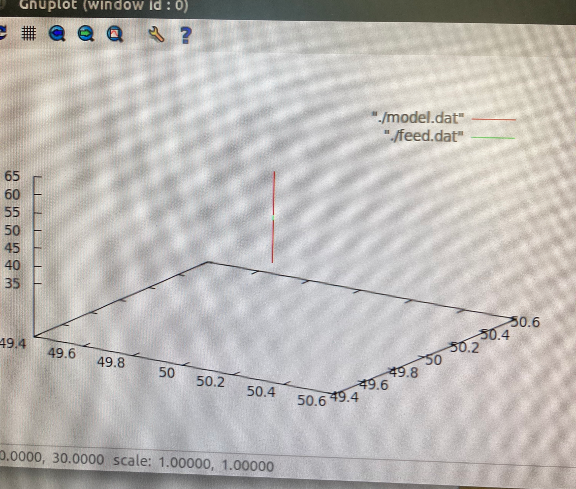
\includegraphics[scale=0.4]{fg1.png}
  \caption{モデリング}\label{fig:図1}
\end{figure}

\subsection{シミュレーション結果}

\subsubsection{VSWR}
下の図2は半波長ダイポールアンテナのVSWRを表したものである。
\begin{figure}[H]
  \centering
  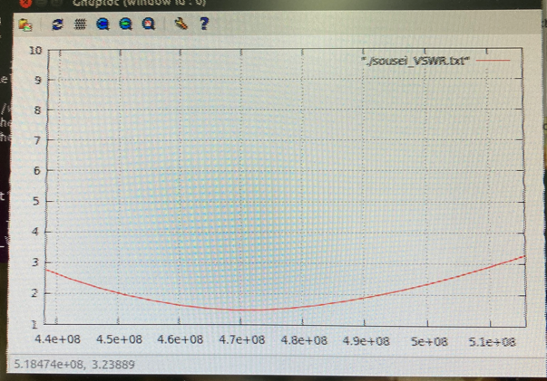
\includegraphics[scale=0.4]{fg2.png}
  \caption{VSWR}\label{fig:図2}
\end{figure}

\end{document}